\documentclass{article}[12 pt]
\usepackage{amssymb}
\usepackage{amsthm}
\usepackage{amsmath}
\usepackage{appendix}
\usepackage{array}
\usepackage{geometry}
\usepackage{enumitem}
\usepackage{graphicx}
\usepackage{subfig}
\usepackage{caption}
\usepackage{url}
\usepackage{float}
\usepackage{pdfpages}
\usepackage{shortvrb}
\usepackage{mathtools}
\usepackage{multirow}
\usepackage{hyperref}
\usepackage{commath}
\usepackage{bm}
\usepackage{tabularx}


\def\BibTeX{{\rm B\kern-.05em{\sc i\kern-.025em b}\kern-.08em
		T\kern-.1667em\lower.7ex\hbox{E}\kern-.125emX}}


\graphicspath{{"/media/edrive/Bayesian_Methods/BHM_Assignments/HW03/Report/Images/"}}
\geometry{margin=1 in}

\newcommand{\smallvskip}{\vspace{5 pt}}
\newcommand{\medvskip}{\vspace{30 pt}}
\newcommand{\bigvskip}{\vspace{100 pt}}
\newcommand{\tR}{\mathtt{R}}




\begin{document}
	
\begin{center}
	\textbf{\Large Connor McCurley} \\
	AGR 6932  \qquad \quad \quad \textbf{\large Homework 3} \quad \quad \qquad Fall 2019 
\end{center}


%===================================================
%=================== Question 1 ====================
%===================================================

\section*{Question 1}
Question 1 demonstrated the effects of partial pooling in hierarchical models.  Given the 8 Schools model, expressed as:

\begin{align*}
	y_i &\sim Normal(\theta_i, \sigma_i) \\
	\theta_i &\sim Normal(\nu, \tau)
\end{align*}

\noindent
we were asked to analyze the partially pooled estimates of treatment for each school, $\theta_i$, as a function of the uncertainty of the global effect, $\tau$. Two cases were considered.  In the first case (Figure \ref{fig:q1_p1}) the prior on $\tau$ was considered as ``uninformative''.  The diagram demonstrates the evolution of the estimates for fixed values of $\tau$.  (Each line represents a single $\theta_i$ estimate.)  As can be seen from Figure \ref{fig:q1_p1}, the $\theta_i$ values converge to their assumed values as the variance, $\tau$, increases.  As discussed in class, this demonstrates the trend from complete pooling (for small $\tau$ values) to no pooling.

\begin{center}
	\begin{figure}[H]
		\centering
		\includegraphics[width=0.6\textwidth]{"q1_p1"}
		\caption{$\Theta_i$ as a function of its variance with an uninformative prior.  Each line represents a particular school from the 8 Schools model.  Complete pooling is demonstrated for small values of $\tau$, while no pooling is observed for larger values.}
		\label{fig:q1_p1}
	\end{figure}
\end{center}

\noindent
A half-normal prior was then placed on $\tau$ and the simulations were repeated for different amounts of variation.  As can be seen in Figure \ref{fig:q1_p2}, the same trend can be observed as with Figure \ref{fig:q1_p1}.  However, it is assumed that more samples are needed for the model to average over the prior.

\begin{center}
	\begin{figure}[H]
		\centering
		\includegraphics[width=0.6\textwidth]{"q1_p2"}
		\caption{$\Theta_i$ as a function of its variance with a half-normal prior.  Each line represents a particular school from the 8 Schools model.  Complete pooling is demonstrated for small values of the variance on $\tau$, while no pooling is observed for larger values.}
		\label{fig:q1_p2}
	\end{figure}
\end{center}

%===================================================
%=================== Question 2 ====================
%===================================================
\section*{Question 2}
Question 2 then asked about varying logistic growth rate processes.  Figure \ref{fig:q2_p1_no_error} shows logistic growth trajectories for 3 different rate parameters, R.  It can be observed that the processes evolve smoothly as N increases.  Figure \ref{fig:q2_p2_process_w_obs_error_2} then shows the same trajectories with added normal observation error.  As can be observed, the trajectories are significantly more chaotic.


\begin{center}
	\begin{figure}[H]
		\centering
		\includegraphics[width=0.6\textwidth]{"q2_p1_no_error"}
		\caption{Logistic growth trajectories for three rate values, 0.1, 0.5, and 1.}
		\label{fig:q2_p1_no_error}
	\end{figure}
\end{center}

\begin{center}
	\begin{figure}[H]
		\centering
		\includegraphics[width=0.6\textwidth]{"q2_p2_process_w_obs_error_2"}
		\caption{Logistic growth trajectories for three rate values, 0.1, 0.5, and 1 with additional normally-distributed observation error.  The error variance was specified as $\sigma_{obs}=2$.}
		\label{fig:q2_p2_process_w_obs_error_2}
	\end{figure}
\end{center}

\noindent
Stan models were then implemented in order to estimate model parameters for the rate, $r$, and observation noise variance, $\sigma_{obs}$.   The following plots demonstrate sample paths for 3 different $r$ values, as well as histograms for the estimates of $r$ and $\sigma_{obs}$.  Simulations were conducted using 6 chains and 1000 samples each.


%====================== r = 0.1 ========================
\begin{center}
	\begin{figure}[H]
		\centering
		\includegraphics[width=0.4\textwidth]{"q3_data_r_point_1"}
		\caption{Logistic growth sample path for $r=0.1$ and $\sigma_{obs}=2$.}
		\label{fig:q3_data_r_point_1}
	\end{figure}
\end{center}

\begin{figure}[H]%
	\centering
	\subfloat[Histogram of $r$ estimates.  The histogram's mean is around 0.07, while the true value is 0.1]{{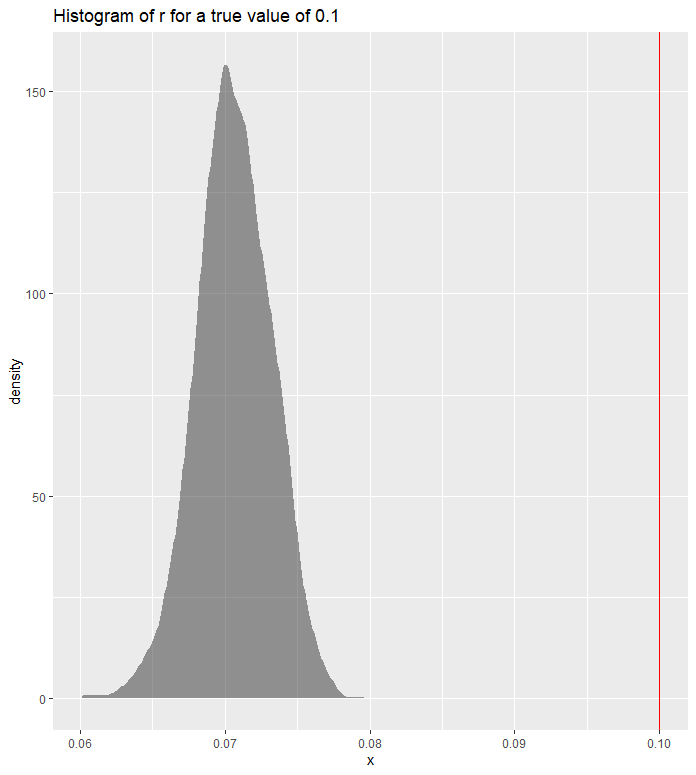
\includegraphics[width=5cm]{q3_r_hist_r_point_1} }}%
	\qquad
	\subfloat[Histogram of $\sigma_{obs}$ estimates.  The histogram's mean is around 2.5, while the true value is 2.0]{{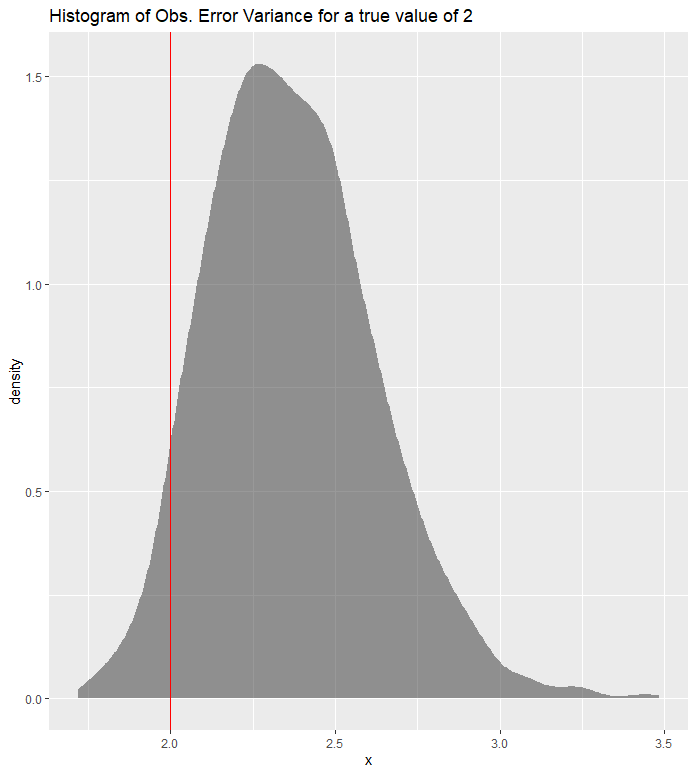
\includegraphics[width=5cm]{q3_obs_error_hist_r_point_1} }}%
	\label{fig:q3_hist_point_1}%
\end{figure}

%====================== r = 0.5 ========================
\begin{center}
	\begin{figure}[H]
		\centering
		\includegraphics[width=0.3\textwidth]{"q3_data_r_point_5"}
		\caption{Logistic growth sample path for $r=0.5$ and $\sigma_{obs}=2$.}
		\label{fig:q3_data_r_point_5}
	\end{figure}
\end{center}

\begin{figure}[H]%
	\centering
	\subfloat[Histogram of $r$ estimates.  The histogram's mean is around 0.47, while the true value is 0.5]{{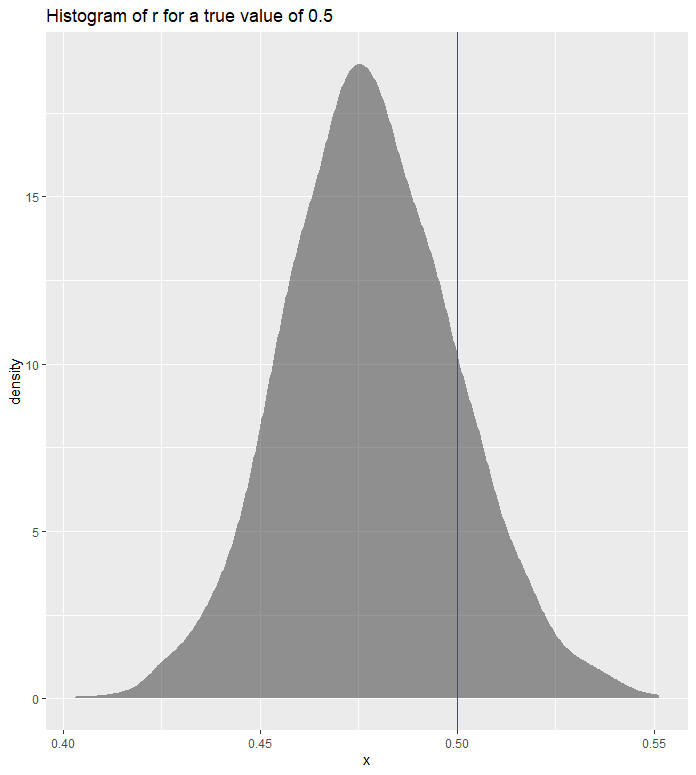
\includegraphics[width=5cm]{q3_r_hist_r_point_5} }}%
	\qquad
	\subfloat[Histogram of $\sigma_{obs}$ estimates.  The histogram's mean is around 2.6, while the true value is 2.0]{{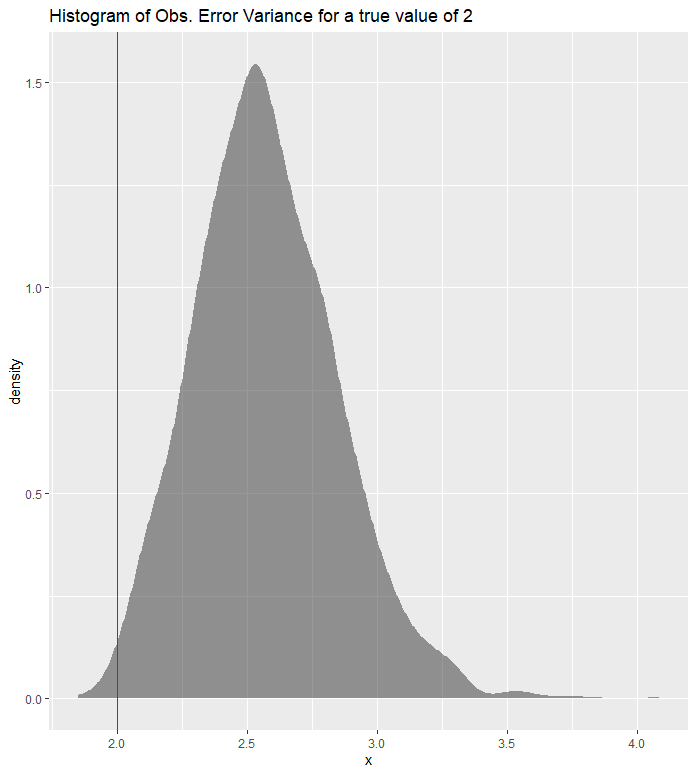
\includegraphics[width=5cm]{q3_obs_error_hist_r_point_5} }}%
	\label{fig:q3_hist_point_5}%
\end{figure}

%====================== r = 1 ========================
\begin{center}
	\begin{figure}[H]
		\centering
		\includegraphics[width=0.4\textwidth]{"q3_data_r_1"}
		\caption{Logistic growth sample path for $r=1$ and $\sigma_{obs}=2$.}
		\label{fig:q3_data_r_1}
	\end{figure}
\end{center}

\begin{figure}[H]%
	\centering
	\subfloat[Histogram of $r$ estimates.  The histogram's mean is around 0.105, while the true value is 1]{{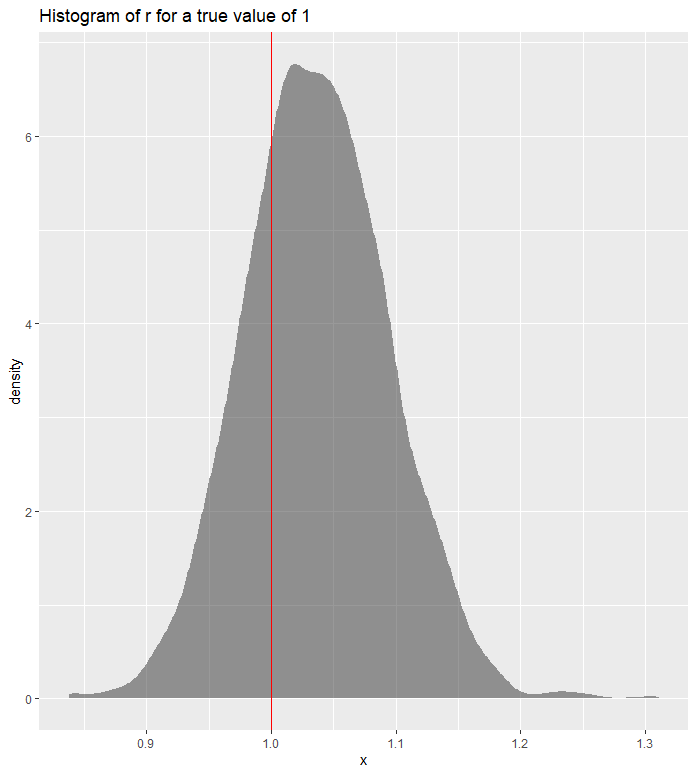
\includegraphics[width=5cm]{q3_r_hist_r_1} }}%
	\qquad
	\subfloat[Histogram of $\sigma_{obs}$ estimates.  The histogram's mean is around 2.4, while the true value is 2.0]{{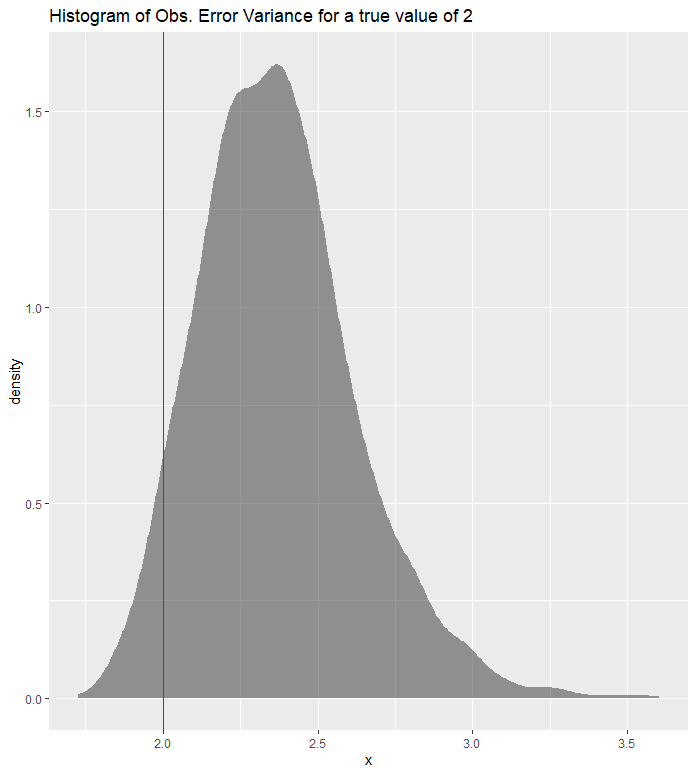
\includegraphics[width=5cm]{q3_obs_error_hist_r_1} }}%
	\label{fig:q3_hist_1}%
\end{figure}

\noindent
It can be observed that the estimates for $r$ became more precise as $r$ increased.

%===================================================
%=================== Question 3 ====================
%===================================================
\newpage
\section*{Question 3}
Question 3 was an extension of question 2, where gamma-distributed process error was added to the models.  Figures \ref{fig:q4_sample_paths_proc_error_only}, \ref{fig:q4_sample_paths_proc_error_and_obs_error}, and \ref{fig:q4_sample_paths_proc_error_and_fixed_obs_error} demonstrate 6 different sample paths for the logistic growth with process error only, process error and observation error, and process error with a fixed observation error.  The process error was kept small, as the model would blow-up otherwise.
  
\begin{center}
	\begin{figure}[H]
		\centering
		\includegraphics[width=0.6\textwidth]{"q4_sample_paths_proc_error_only"}
		\caption{Logistic growth with gamma-distributed process error.  The parameters of the model were set as $r=0.5$, $K=100$, and $dK=0.25$ (dispersion constant).}
		\label{fig:q4_sample_paths_proc_error_only}
	\end{figure}
\end{center}

\begin{center}
	\begin{figure}[H]
		\centering
		\includegraphics[width=0.6\textwidth]{"q4_sample_paths_proc_error_and_obs_error"}
		\caption{Logistic growth with gamma-distributed process error and normally-distributed observation error.  The parameters of the model were set as $r=0.5$, $K=100$, $dK=0.25$ (dispersion constant), and $\sigma_{obs}=2$.}
		\label{fig:q4_sample_paths_proc_error_and_obs_error}
	\end{figure}
\end{center}

\begin{center}
	\begin{figure}[H]
		\centering
		\includegraphics[width=0.6\textwidth]{"q4_sample_paths_proc_error_and_fixed_obs_error"}
		\caption{Logistic growth with gamma-distributed process error and normally-distributed observation error.  The parameters of the model were set as $r=0.5$, $K=100$, $dK=0.25$ (dispersion constant), and fixed $\sigma_{obs}=0.8$.}
		\label{fig:q4_sample_paths_proc_error_and_fixed_obs_error}
	\end{figure}
\end{center}

\noindent
At this point, I mostly implemented the code to run the Stan models.  However, I had difficulty getting it to actually sample.  (Unfortunately, I did not have a lot of time to investigate due to my upcoming project status meeting.)


\end{document}
